\documentclass[sigconf,review]{acmart}

\usepackage{booktabs} % For formal tables
\usepackage{subfigure}
\usepackage{url}

% Copyright
\setcopyright{none}
%\setcopyright{acmcopyright}
%\setcopyright{acmlicensed}
%\setcopyright{rightsretained}
%\setcopyright{usgov}
%\setcopyright{usgovmixed}
%\setcopyright{cagov}
%\setcopyright{cagovmixed}


% DOI
\acmDOI{10.475/123_4}

% ISBN
\acmISBN{123-4567-24-567/17/06}

%Conference
\acmConference[SIGGRAPH 2017 Posters]{SIGGRAPH 2017 Posters}{August 2017}{Los Angeles, CA, USA} 
\acmYear{2017}
\copyrightyear{2017}
\acmPrice{15.00}

% use the "authoryear" citation style.
\citestyle{acmauthoryear}
\setcitestyle{square}

\begin{document}
\title{New Features for GRNsight v2: a web application and service for visualizing models of small- to medium-scale gene regulatory networks}

\author{Eileen J. Choe}
\orcid{0002-8116-9224}
\affiliation{
  \institution{Loyola Marymount University \\ Department of Electrical Engineering and Computer Science}
  \streetaddress{1 LMU Drive}
  \city{Los Angeles} 
  \state{California} 
  \postcode{90045}
}
\email{echoe@lion.lmu.edu}

\author{Nicole A. Anguiano}
\affiliation{
 \institution{Loyola Marymount University \\ Department of Electrical Engineering and Computer Science}
  \streetaddress{1 LMU Drive}
  \city{Los Angeles} 
  \state{California} 
  \postcode{90045}
}
\email{TBD}

\author{Anindita Varshneya}
\affiliation{
 \institution{Loyola Marymount University \\Department of Biology}
  \streetaddress{1 LMU Drive}
  \city{Los Angeles} 
  \state{California} 
  \postcode{90045}
}
\email{TBD}

\author{Mihir Samdarshi}
\affiliation{
 \institution{Loyola Marymount University \\Department of Biology}
  \streetaddress{1 LMU Drive}
  \city{Los Angeles} 
  \state{California} 
  \postcode{90045}
}
\email{TBD}

\author{Yeon-Soo Shin}
\affiliation{
 \institution{Loyola Marymount University \\Department of Electrical Engineering and Computer Science}
  \streetaddress{1 LMU Drive}
  \city{Los Angeles} 
  \state{California} 
  \postcode{90045}
}
\email{TBD}

\author{Edward B. Bachoura}
\affiliation{
 \institution{Loyola Marymount University \\Department of Electrical Engineering and Computer Science}
  \streetaddress{1 LMU Drive}
  \city{Los Angeles} 
  \state{California} 
  \postcode{90045}
}
\email{TBD}

\author{John David N. Dionisio}
\affiliation{
 \institution{Loyola Marymount University \\Department of Electrical Engineering and Computer Science}
  \streetaddress{1 LMU Drive}
  \city{Los Angeles} 
  \state{California} 
  \postcode{90045}
}
\email{TBD}


\author{Kam D. Dahlquist}
\affiliation{
 \institution{Loyola Marymount University \\Department of Biology}
  \streetaddress{1 LMU Drive}
  \city{Los Angeles} 
  \state{California} 
  \postcode{90045}
}
\email{TBD}


% The default list of authors is too long for headers}
\renewcommand{\shortauthors}{B. Trovato et. al.}

\begin{abstract}

We present new features in v2 of GRNsight, a web application and service for interactive visualization of small- to medium-scale gene regulatory networks (GRNs) \cite{peerj}. A GRN consists of genes, transcription factors, and the regulatory connections between them which govern the level of expression of mRNA and protein from genes. GRNsight produces weighted or unweighted network graphs from an Excel spreadsheet containing an adjacency matrix where regulators are named in the columns and target genes in the rows, a Simple Interaction Format (SIF) text file, or a GraphML XML file. GRNsight represents genes as nodes and regulatory connections as edges with colors, end markers, and thicknesses corresponding to the sign and magnitude of activation or repression. For GRNsight v2, the user was given greater control over the network visualization's bounding box and viewport as well as the way edges and their weights are displayed. GRNsight is best-suited for visualizing networks of fewer than 35 nodes and 70 edges, and has general applicability for displaying any small, unweighted or weighted network with directed edges for systems biology or other application domains. The GRNsight application (\url{http://dondi.github.io/GRNsight/}) and code (\url{https://github.com/dondi/GRNsight}) are available under the open source BSD license.

\end{abstract}

%
% The code below should be generated by the tool at
% http://dl.acm.org/ccs.cfm
% Please copy and paste the code instead of the example below. 
%
\begin{CCSXML}
<ccs2012>
<concept>
<concept_id>10003120.10003145.10003147.10010364</concept_id>
<concept_desc>Human-centered computing~Scientific visualization</concept_desc>
<concept_significance>500</concept_significance>
</concept>
<concept>
<concept_id>10003120.10003145.10003151.10011771</concept_id>
<concept_desc>Human-centered computing~Visualization toolkits</concept_desc>
<concept_significance>500</concept_significance>
</concept>
</ccs2012>
\end{CCSXML}

\ccsdesc[500]{Human-centered computing~Scientific visualization}
\ccsdesc[500]{Human-centered computing~Visualization toolkits}

% We no longer use \terms command
%\terms{Theory}

\keywords{Scientific Visualization, Software Engineering, Bioinformatics}

\begin{teaserfigure}
    \centering
    \subfigure[Screenshot of GRNsight]
    {
        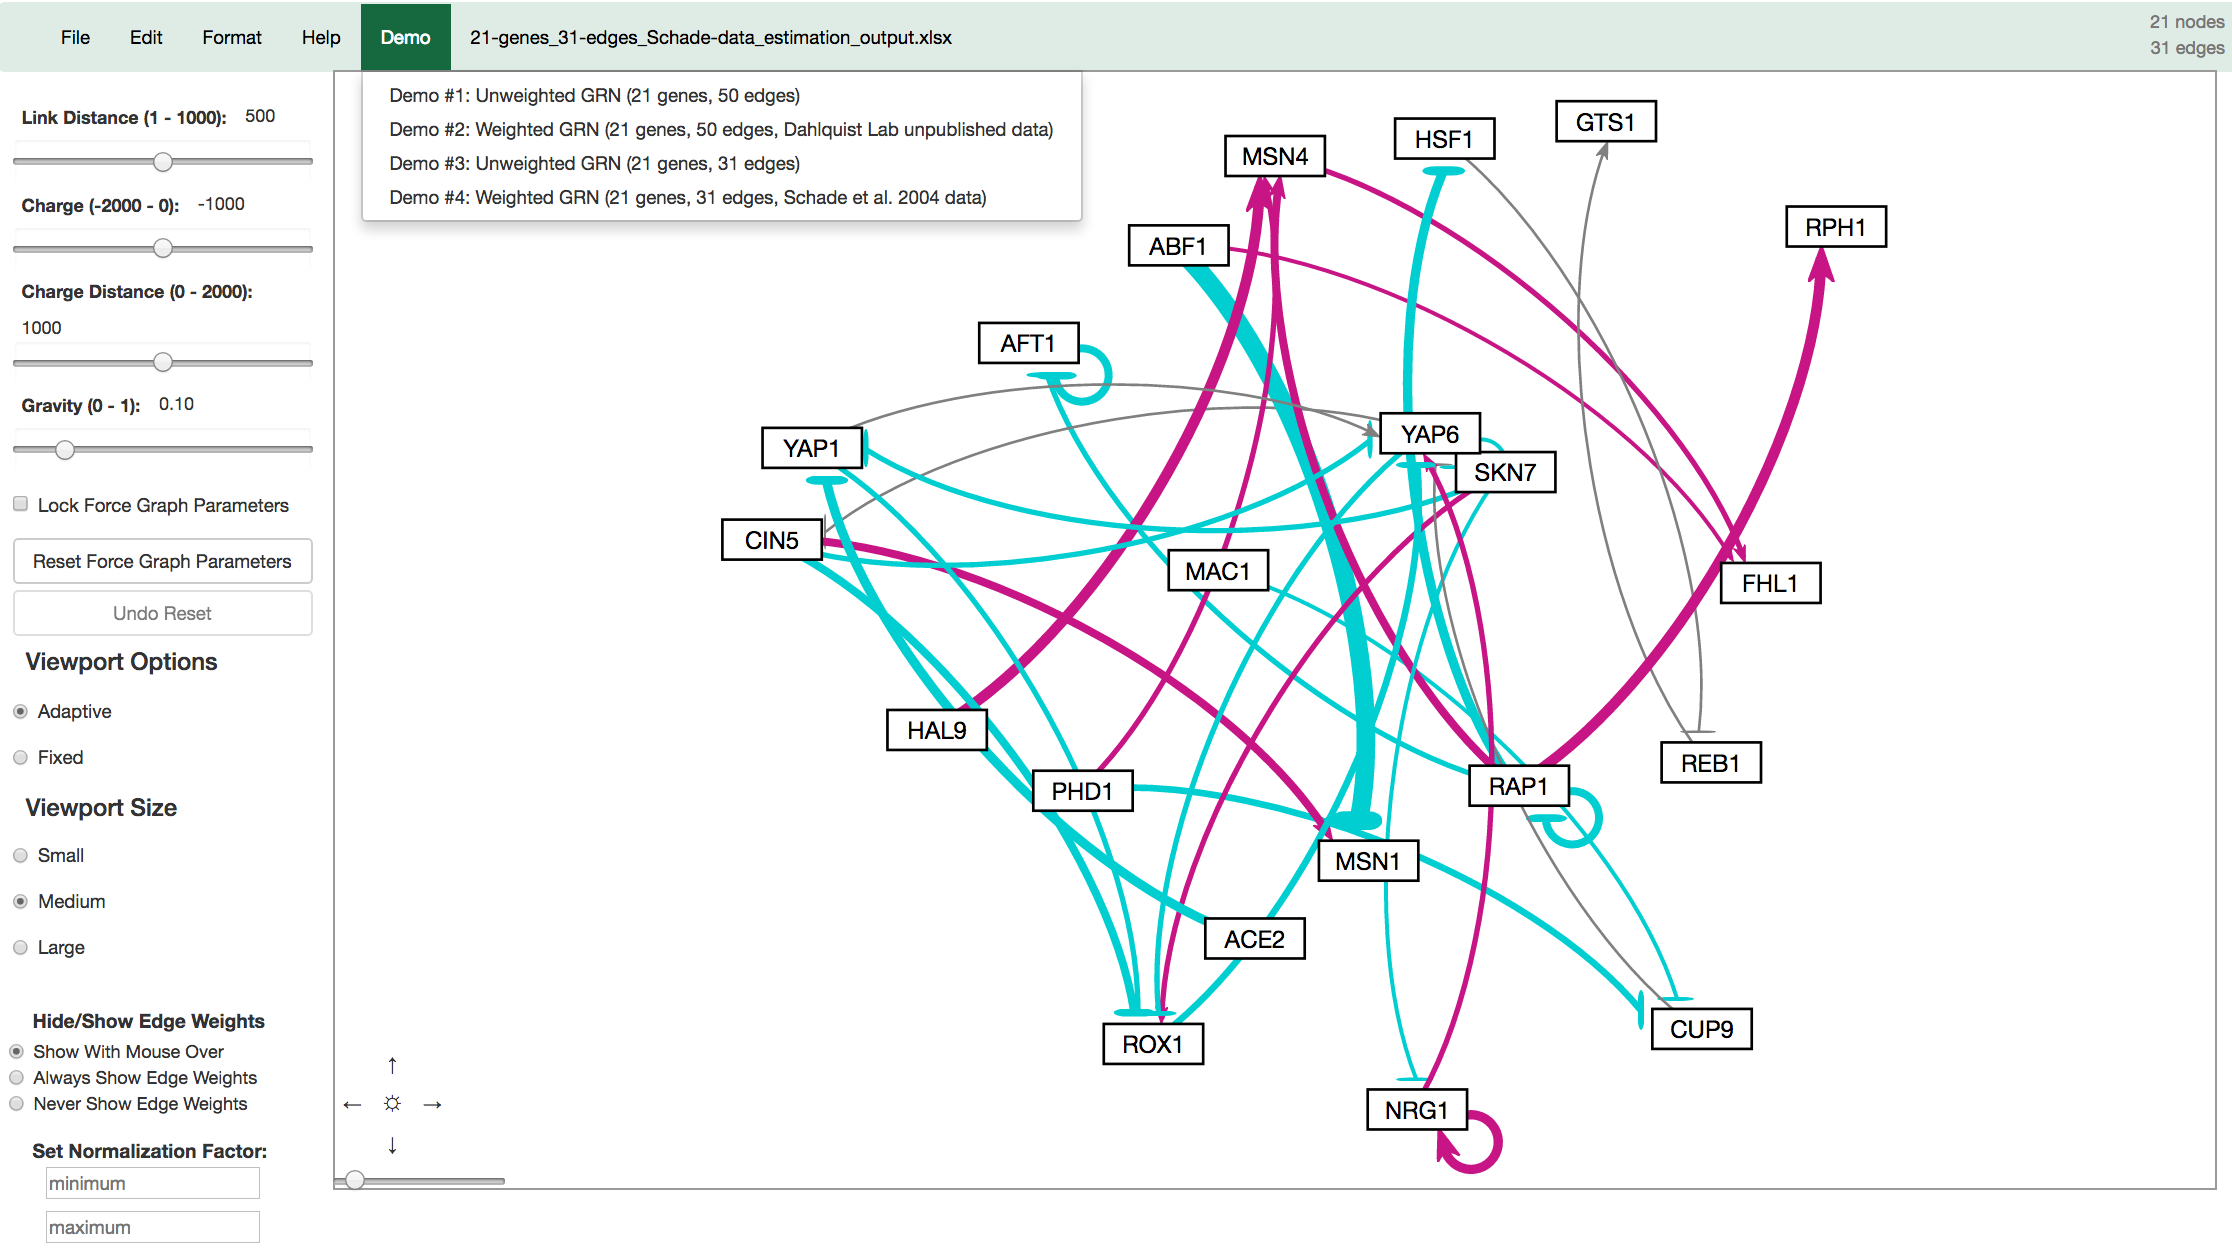
\includegraphics[height=1.5in]{screenshot-auto.png}
        \label{fig:full-screenshot}
    }
    \subfigure[Weighted graph after manual manipulation.]
    {
        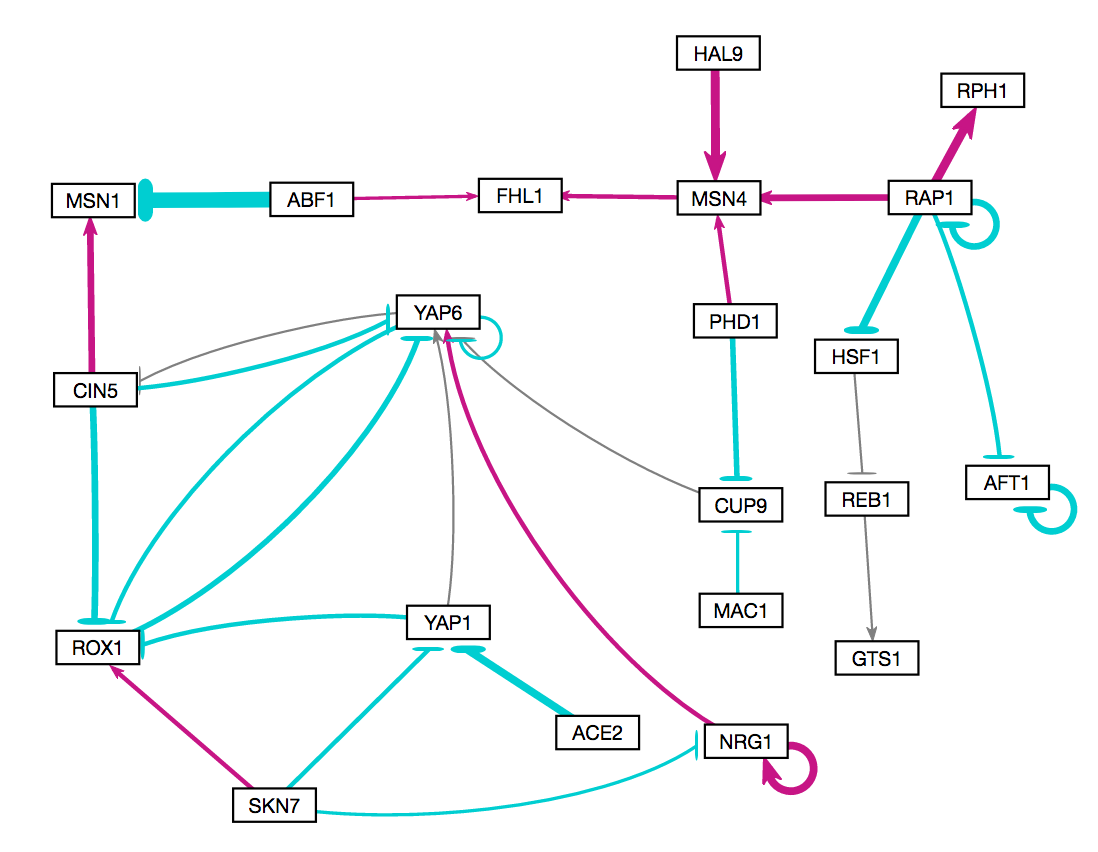
\includegraphics[height=1.5in]{never-weights.png}
        \label{fig:no-weights}
    }
    \subfigure[Weighted graph with edge weights displayed.]
    {
        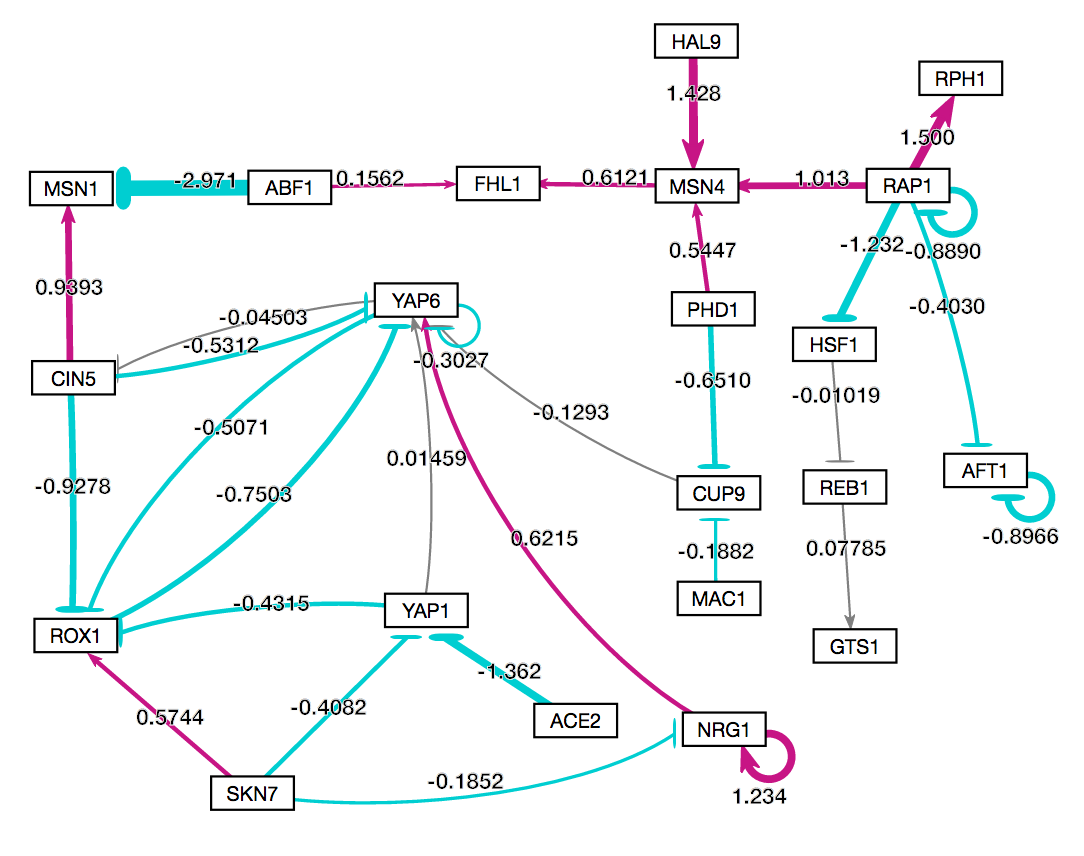
\includegraphics[height=1.5in]{always-weights.png}	
        \label{fig:with-weights}
    }
    \caption{GRNsight v2's automatic graph layout of Demo \#4: Weighted GRN (21 genes, 31 edges, Schade et al. 2004 data) in (a) allows the demo gene regulatory network to fully relax. Zooming and scrolling options allow the user to see the entire graph when it moves beyond the viewport; (b) the user can manipulate the display of the graph through manual node dragging, and can either hide (b), or show (c) all the weight values, which display on the edges.
    }
    \label{fig:screenshots}
\end{teaserfigure}

\maketitle

\section{Introduction and Motivation}

GRNsight is a web application and service for the interactive visualization of small- to medium-scale gene regulatory networks (GRNs), optimized for use by novice and experienced biologists alike to quickly and easily view unweighted and weighted network graphs \cite{peerj}. Visual inspection has long been recognized as distinct from other forms of purely numeric, computational, or algorithmic data analysis \cite{Tufte:1986:VDQ:33404, card1999readings}, and GRNsight enables the potential for insight derived specifically by visual inspection. The following are the requirements for GRNsight:

\begin{enumerate}
\item Exist as a web application without the need to download and install specialized software;
\item Be simple and intuitive to use;
\item Automatically lay out and display small- to medium-scale, unweighted and weighted, directed network graphs in a way that is familiar to biologists and adds value to the interpretation of the modeling results.
\end{enumerate} 

\textbf{Software Architecture}: GRNsight has a service-oriented architecture, consisting of separate server and web client components The server provides a web API that accepts files in Microsoft Excel workbook (.xlsx), SIF (.sif), and GraphML (.graphml) formats and converts them into a unified JSON representation. A converse import function accepts this JSON representation and converts it into either SIF (.sif) or GraphML (.graphml) formats for export. The web application server provides code and resources for the graphical user interface that displays this JSON representation of the graph.\\

\textbf{Graph Customizations and User Interface}: Graph visualization is facilitated by the Data-Driven Documents JavaScript library \cite{d3}. D3.js provides data mapping and layout routines which GRNsight heavily customizes in order to achieve the desired graph visualization. The resulting graph is a Scalable Vector Graphics (SVG) drawing in which D3.js maps gene objects from the JSON representation provided by the web API server onto labeled rectangles. Edge weights are mapped into Bezier curves. The resulting graph is interactive, initially using D3.js's force graph layout algorithm to automatically determine the positions of the gene rectangles. The GRNsight user interface includes a menu/status bar and sliders that adjust D3.js's force graph layout parameters, to refine the automated visualization. Design decisions for the user interface were driven by applicable interaction design guidelines and principles \cite{norman2013design,shneiderman2010designing,nielsen1994usability} in alignment with the mental model and expectations of the target user base, consisting primarily of biologists.

\section{Extensions to GRNsight in v2}
Since the release of GRNsight v1, further research, as well as feature requests from peer review have motivated the following improvements to GRNsight v2. We focus on features which have enhanced the visualization and display of the network graph GRNsight produces.

\subsection{Separation of Viewport from Graph Bounding Box}

The default behavior of D3.js's force graph layout algorithm is to give the graph an a priori bounding box. To accommodate the range of possible GRNs that GRNsight may display, we revised that algorithm so that the option for an adaptive, expandable bounding box can be chosen.

\begin{enumerate}
  \item The bounding box can now be fixed to the size of the viewport or adapted to the size of the graph
  \item The viewport size can be selected from among small, medium, and large options
  \item The best viewport size is automatically detected from the browser
  \item The viewport can be fit to the size of the browser window 
  \item Zooming and scrolling have been enabled
\end{enumerate}


\subsection{Edge Weight Display Options}
A new visualization feature for weighted graphs introduced in GRNsight v2 is an options menu for displaying the edge weights of the graph. By default, edge weights are shown only upon mouse-over of the edge. Users can now choose to always show or always hide weights. Edge Options exist in the sidebar menu, and under the Format tab in the File menu.

\subsection{Graph Normalization}
To allow for the comparision of weighted network graphs, a feature request was made for the user to have the option to customize the normalization factor applied to the edge thickness of the graph. By default, GRNsight detects the maximum and minimum relationship values of a network, and normalizes the data to fit within 12 distict edge thicknesses corresponding to the strength of its regulatory relationship. By adding the option to user-specified minimum and maximum values, the edge thicknesses can be consistently normalized in a weighted graph, so the user can compare different graphs on the same scale. 

\section{Conclusion and Future Work}
We have successfully implemented GRNsight, a web application and service for visualizing small- to medium-scale GRNs that is simple and intuitive to use. GRNsight reads a weighted or unweighted representation of a GRN, and automatically lays out and displays unweighted and weighted network graphs, enabling interpretation of the weight parameters more easily than one could from an adjacency matrix alone. Extensions to GRNsight in v2 have expanded GRNsight's visualization and layout capababilities, giving the user more control over the visual display of the network graph.

GRNsight is in active development, we would like to further enhance the tool to compute and display graph statistics, as betweenness centrality measure. Further research will be conducted to evaluate different graph layout options, such as a hierarchical or block layout and the effectiveness that alternate visualization paradigms for the biologist...

\bibliographystyle{ACM-Reference-Format}
\bibliography{siggraph-abstract-review} 

\end{document}
